We performed an end-to-end evaluation of our prototype in our second cluster.
This cluster has 5 test nodes, and is connected to
a 5-shelves PanFS storage cluster with 5 metadata nodes and 50 storage nodes.
Each test node has 64 cores and is using 40GE NIC, which are enough
to saturate the data bandwidth of our PanFS storage cluster.
Because of some technique difficulties,
we did not run our GIGA+ server processes inside the metadata node.
Instead, we co-locate our GIGA+ server processes
with client processes in the test nodes.
Each test node runs a GIGA+ server that is assigned to a metadata node
as explained in Section \ref{design.integration}.
We ran a series of HPC benchmark runs using the open source \textit{mdtest}
synthetic benchmark \cite{mdtest}
and File System Test Suite checkpoint benchmark from LANL \cite{mpiio}
to test metadata path and data path separately.

\subsubsection*{Metadata Intensive Workloads}
To evaluate the metadata performance of layering on PanFS,
we use mdtest to generate a three-step workload:
The first step, similar to the last one, is to create 5 million
zero-files in a single directory;
the second step is to perform a $stat()$ on random files in the directory;
the third step is to delete all the files in the directory in a random order.
Each step involves multiple clients to issue the operations concurrently.

If we directly use the above workload to directly compare our layered system
against the original PanFS, it would not be fair enough.
This is because a single directory can only use the hardware resource
of one metadata manager in PanFS,
and PanFS also limits a single directory to 1 million files.
Therefore we chose to compare native PanFS creating 1 million files
in 5 different directories owned by 5 different metadata managers.
The total number of clients used for testing the two systems
are kept the same.


\begin{figure}[t]  %%%%%%%%%%%%%%%%%%%%%%%
\centerline{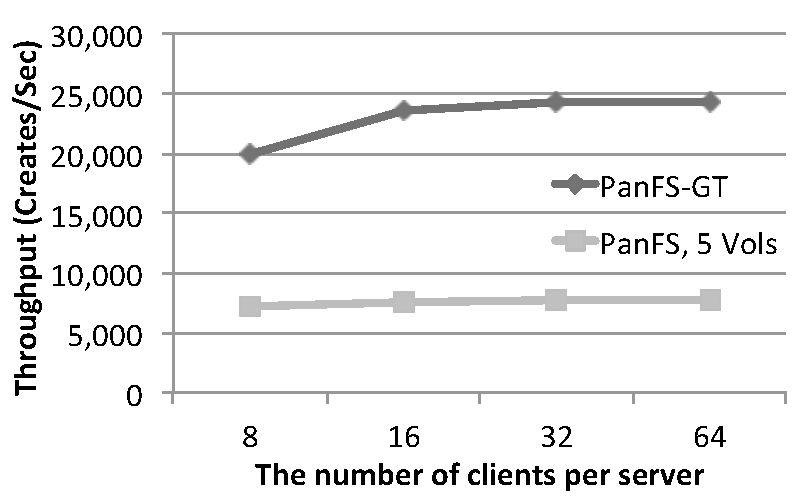
\includegraphics[scale=0.6]{./figs/zero_file_creation_on_panfs}}
\vspace{10pt}
\caption{\normalsize
\textit{Create five million zero-length files in one empty directory
with different number of clients.}
}
\vspace{10pt}
\hrule
\label{graph:creation_clients}
\end{figure}       %%%%%%%%%%%%%%%%%%%%%%%

Figure \ref{graph:creation_clients}

\begin{figure}[t]  %%%%%%%%%%%%%%%%%%%%%%%
\centerline{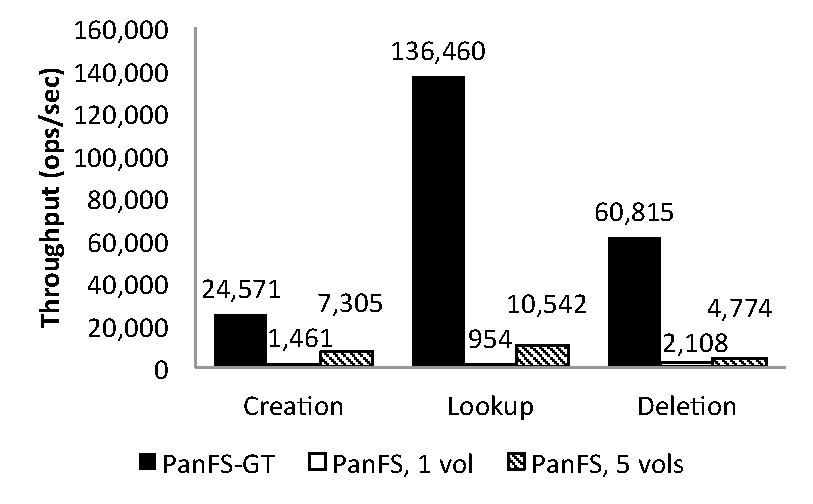
\includegraphics[scale=0.6]{./figs/mdtest}}
\vspace{10pt}
\caption{\normalsize
\textit{mdtest:
The average throughput of different operations in mdtest
when generating 5 million zero-length files in a single shared directory.
Since PanFS has a hard limit to allow only create 1 million entries
in one directory, the bar showing PanFS with 1 volume only gives
the average throughput for the case of creating 1 million entries.
}
}
\vspace{10pt}
\hrule
\label{graph:mdtest_ops}
\end{figure}       %%%%%%%%%%%%%%%%%%%%%%%


\begin{figure}[t]  %%%%%%%%%%%%%%%%%%%%%%%
\centerline{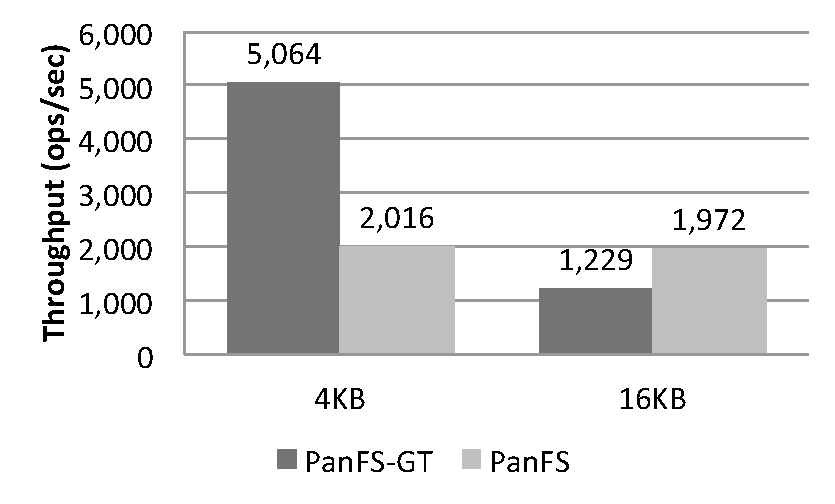
\includegraphics[scale=0.5]{./figs/small_file_creates}}
\vspace{10pt}
\caption{\normalsize
\textit{Create 5 million small files with different size
in one share directory}
}
\vspace{10pt}
\hrule
\label{graph:smallfiles}
\end{figure}       %%%%%%%%%%%%%%%%%%%%%%%

\textbf{Data Intensive Workloads}
%Library version not FUSE
%Clean cache

The LANL filesystem checkpoint benchmark can
generate many types for HPC checkpoint I/O patterns.
For all of our tests, we configured the benchmark to
generate a concurrently written N-N checkpoint.
All checkpoint file I/O is performed by a set of processes
that synchronize with each other using MPI barriers.
In the first phase of the benchmark each process opens the
freshly created checkpoint file for writing and
then waits at a barrier until all nodes are ready to write.
Once all nodes are ready, each node starts
concurrently writing the checkpoint data to its own file.
Each node continues writing to the checkpoint file
until it has written the specified number
of access units, then it waits at an MPI barrier
until all the other nodes have completed writing the data.
Once writing is complete and an MPI barrier reached,
each node syncs its data to disk, closes the file, and then
waits at a file barrier before finishing.
Before starting the read phase we terminate all processes
accessing the underlying file so that
we can unmount the filesystem in order to ensure that
all freshly written data has been flushed from all the nodes'
memory to avoid cached data from unfairly biasing our read performance.
After the filesystem has been mounted and restarted,
the benchmark reads the checkpoint in the same way it was written,
however we shift, so each process will read
the file generated by another process.

\begin{figure}[t]  %%%%%%%%%%%%%%%%%%%%%%%
\centerline{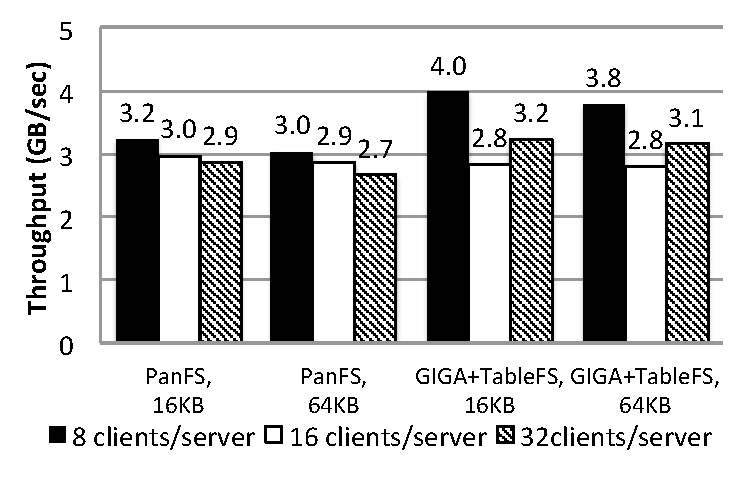
\includegraphics[scale=0.6]{./figs/checkpointing_write}}
\vspace{10pt}
\caption{\normalsize
\textit{
The aggregated write throughput in N-N check-pointing workload.
Each volume receives 640 GB data.
}
}
\vspace{10pt}
\hrule
\label{graph:checkpoint_write}
\end{figure}       %%%%%%%%%%%%%%%%%%%%%%%

\begin{figure}[t]  %%%%%%%%%%%%%%%%%%%%%%%
\centerline{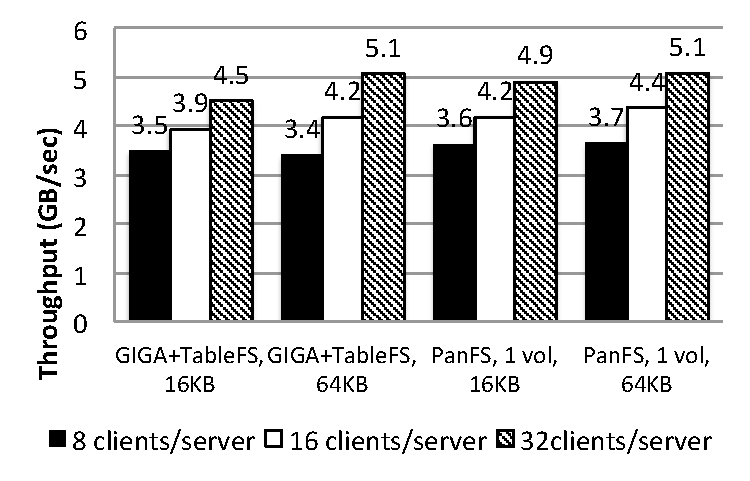
\includegraphics[scale=0.6]{./figs/checkpointing_read}}
\vspace{10pt}
\caption{\normalsize
\textit{
The aggregated read throughput in N-N check-pointing workload.
}
}
\vspace{10pt}
\hrule
\label{graph:checkpoint_read}
\end{figure}       %%%%%%%%%%%%%%%%%%%%%%%

